\section{Implementation}

% TODO: general class structure

\subsection{Class structure}

\begin{figure}[hbt]
  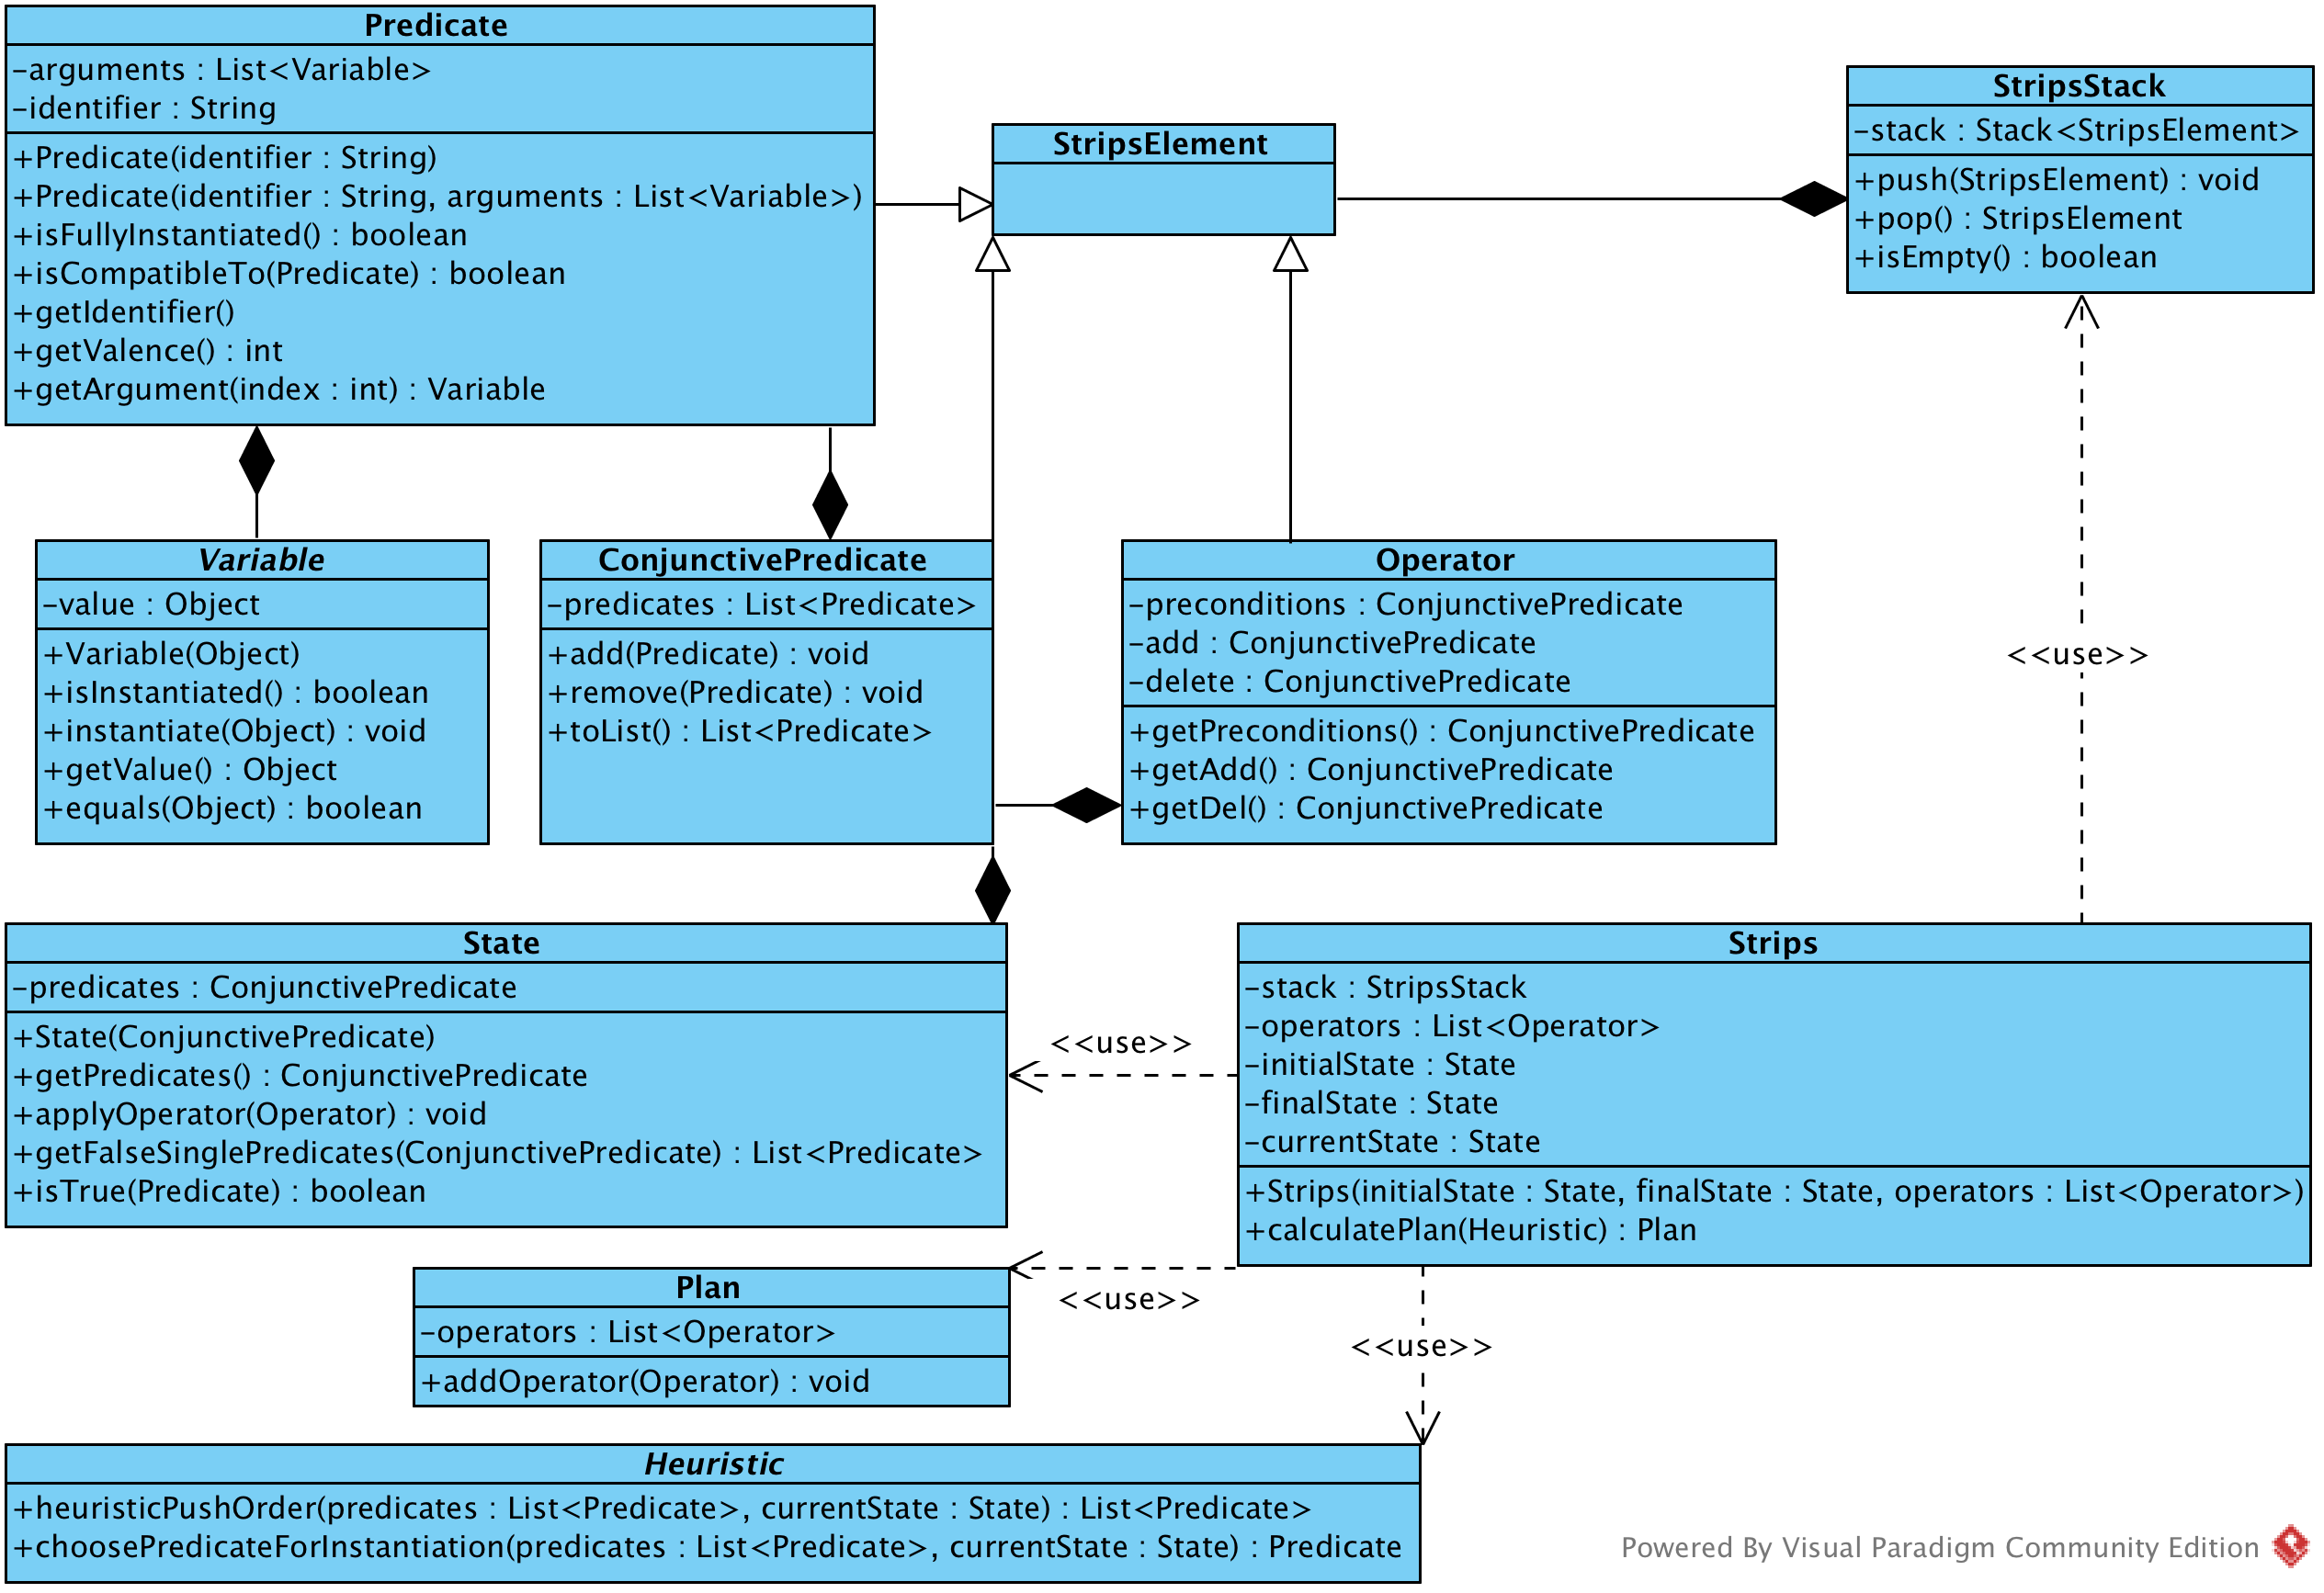
\includegraphics[width=1.1\textwidth]{uml/CD1}
  \caption{UML Class Diagram of STRIPS classes}
\end{figure}

% TODO: specific class strucutre

\subsection{Implementation details}

\begin{lstlisting}[language=Java, caption=Strips method  \textit{instantiate}]
private void instantiate(Predicate singlePred, Heuristic heuristic) {
  List<Predicate> compatiblePredicates = new ArrayList<>();
  for (Predicate currPred : this.currentState.getPredicates().toList()) {
    // find all compatible predicates in current state:
    if (currPred.isCompatibleTo(singlePred)) {
      compatiblePredicates.add(currPred);
    }
  }
  ... 
  // Heuristic chooses one candidate from compatiblePredicates
  Predicate chosenPred = heuristic.choosePredicateForInstantiation(
				compatiblePredicates, currentState);
				
  // instantiate with singlePred with constants of chosenPred
  for (int i = 0; i < chosenPred.getValence(); i++) {
    if (!singlePred.getArgument(i).isInstantiated()) {
      // instantiate updates the java object of the variable.
      // all references to this variable in other predicates
      // will now reference to the instantiated variable.
      singlePred.getArgument(i).instantiate(
                   chosenPred.getArgument(i).getValue());
    }
  } 
}
\end{lstlisting}
